Escribe el valor de la fuerza gravitacional que ejerce una persona de 65
kilogramos en los siguientes cuerpos celestes del Sistema Solar

\begin{multicols}{2}
    \begin{parts}
        \part  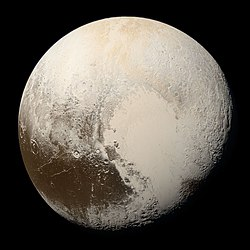
\includegraphics[width=0.8\linewidth]{../images/pluton}
        Pluton\\
        $g=0.62  m/s^2$   \fillin[] N

        \part  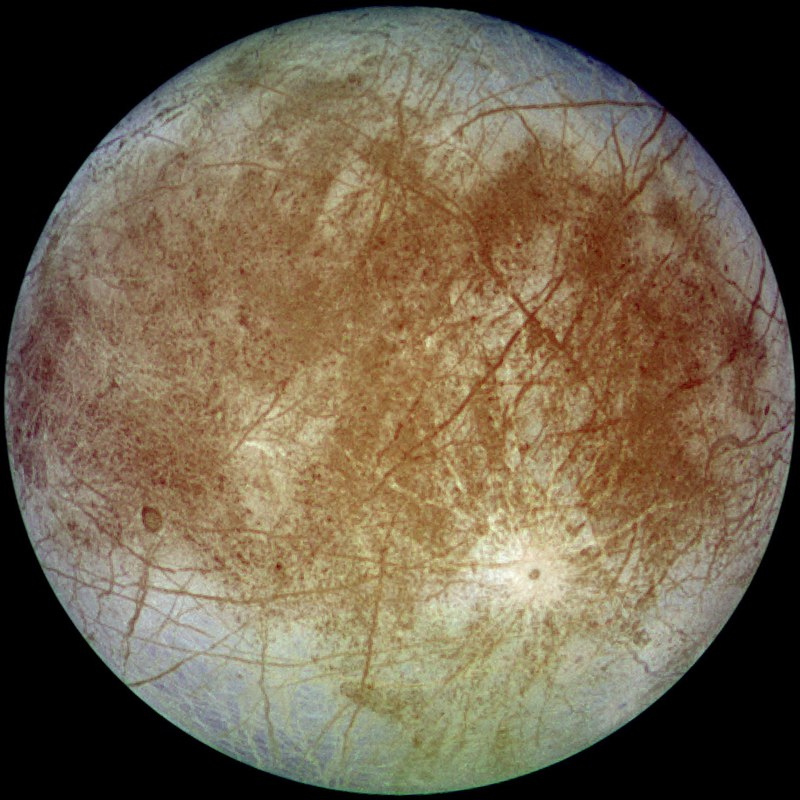
\includegraphics[width=0.8\linewidth]{../images/Europa-moon}

        Europa\\
        $g=1.314  m/s^2$   \fillin[] N

        \part  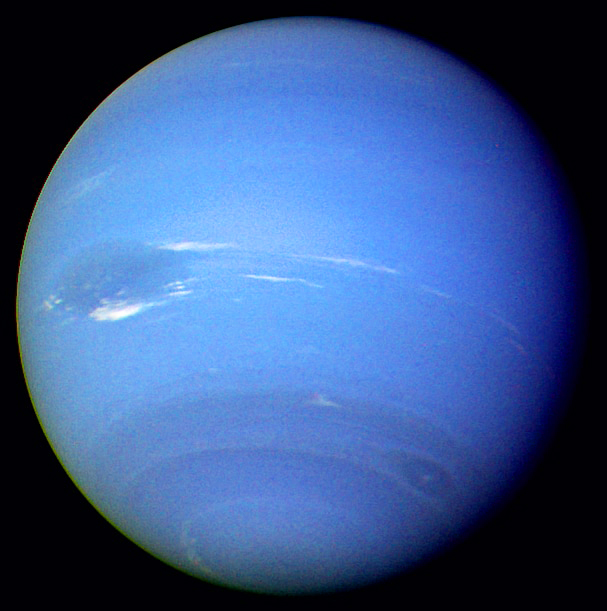
\includegraphics[width=0.8\linewidth]{../images/Neptune}
        Neptuno\\
        $g=11  m/s^2$	\fillin[] N

        \part 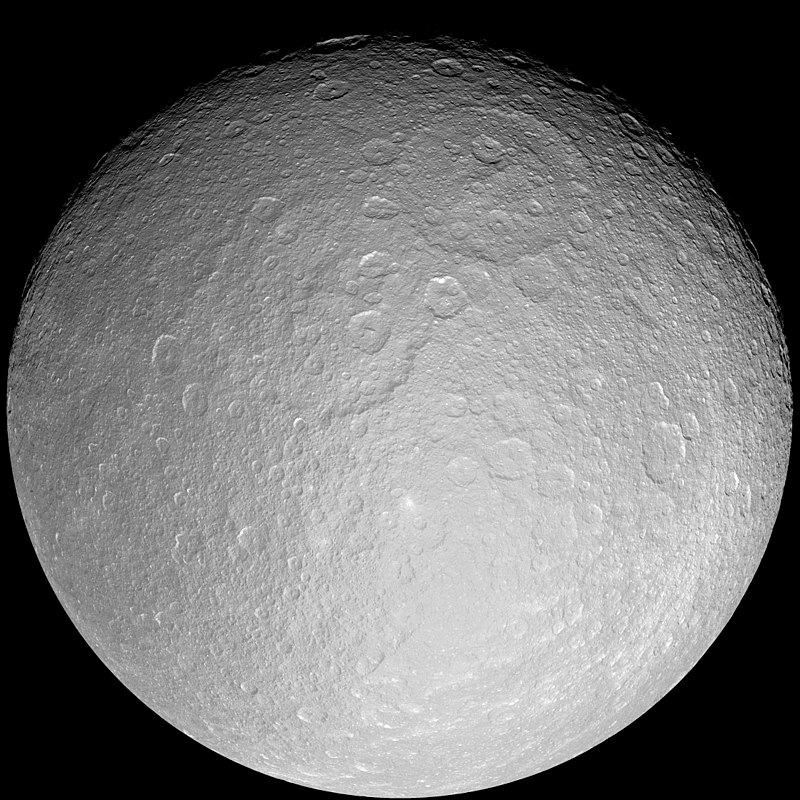
\includegraphics[width=0.8\linewidth]{../images/rea}
        % \begin{minipage}[t][][b]{0.2\textwidth}

        % \end{minipage}\hfill
        % \begin{minipage}[c][][c]{0.5\textwidth}
        Rea\\
        $g=0.264 m/s^2$   \fillin[] N
        % \end{minipage}
    \end{parts}
\end{multicols}